\section{Main Loop}
\label{chapter:implementation:loop}

	The implementation of the render loop designed in Section \ref{chapter:design:loop} is outlined in Figure \ref{fig:TaskGroup}. The \classname{Task} class is the base class for all operations to be performed in-between the rendering steps. The \classname{TaskGroup} combines multiple \classname{Task}s into a single \classname{Task}.

	\begin{figure}[htbp]
		\centering
		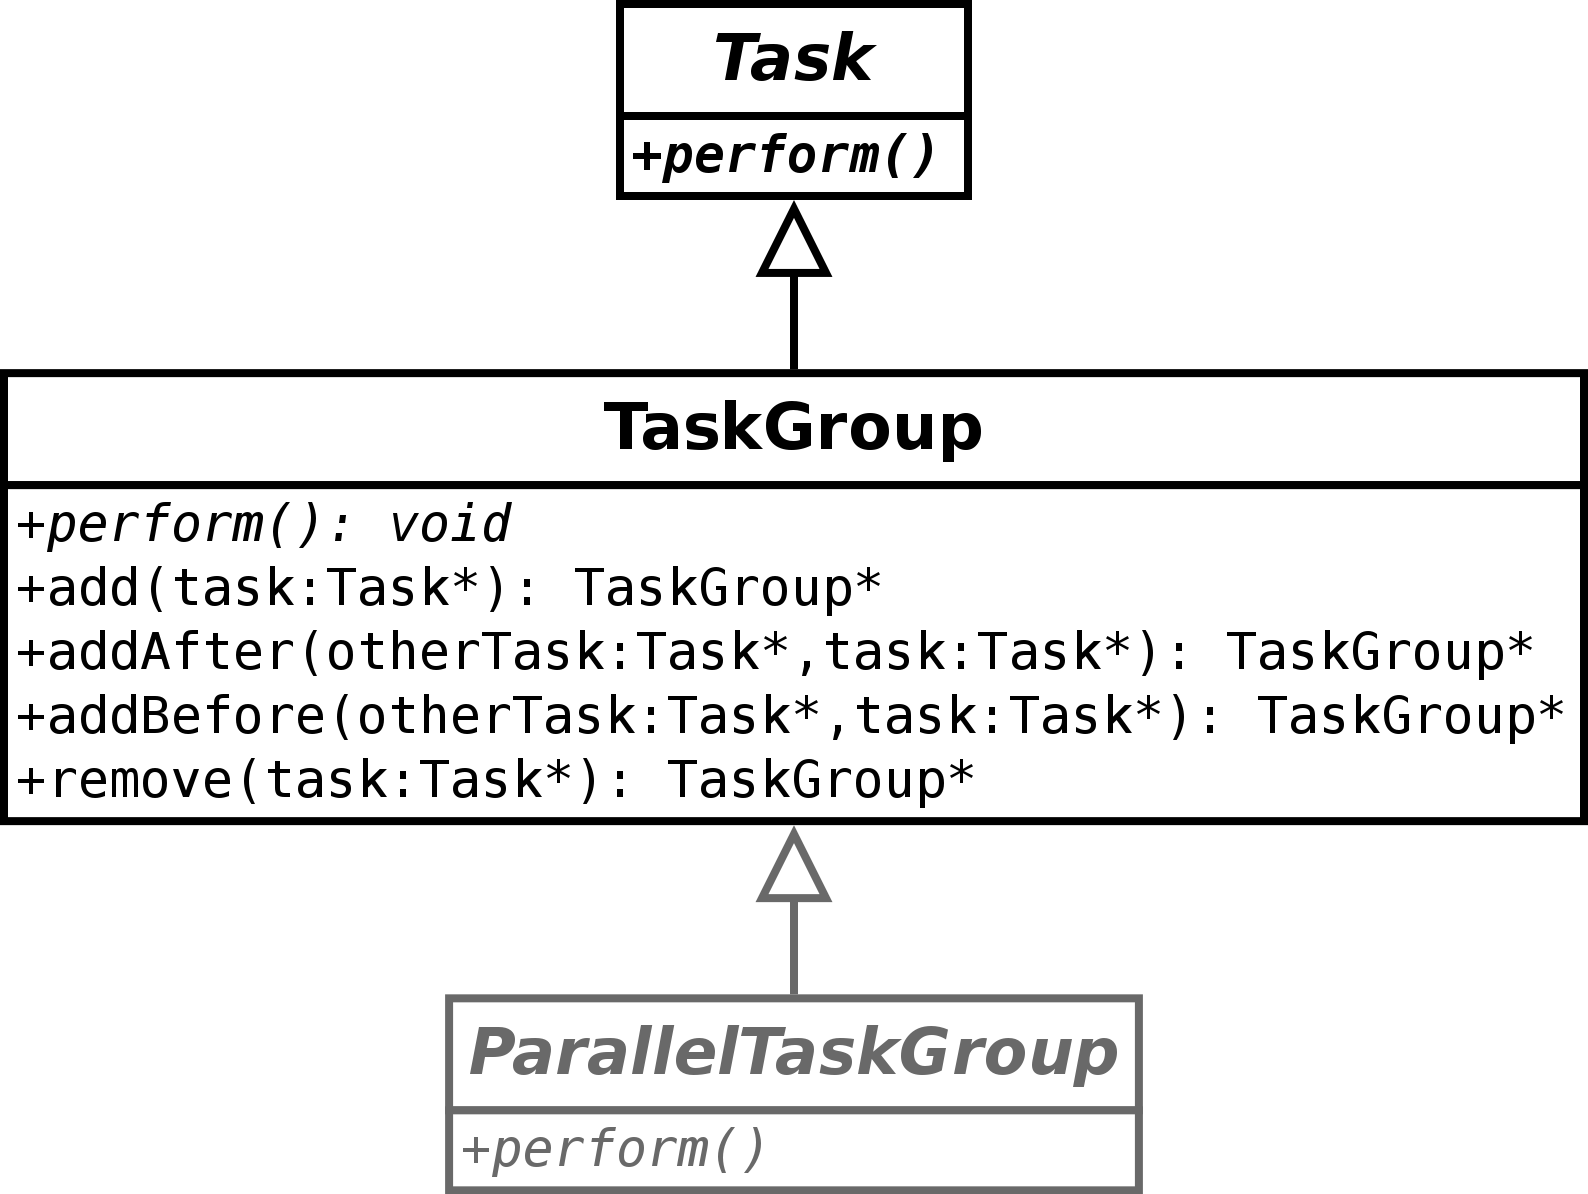
\includegraphics[width=8cm]{images/TaskGroup.png}
		\caption{Outline of the \classname{TaskGroup} class.}
		\label{fig:TaskGroup}
	\end{figure}

	The current implementation of \inlinecode{TaskGroup::perform()} calls all registered \classname{Task}s sequentially. An alternative to this approach would be the implementation of a \classname{ParallelTaskGroup}. This idea was not implemented, though, as this would require the introduction of thread-safety to the application as a whole. This additional option could be pursued at a later time as an optimization technique to the PURGE library.
	
	\subsection{RenderTask}

		PURGE further needs to provide some tasks by itself covering the rendering step. These special tasks are responsible for passing control to any active \classname{GraphicsImplementer} to generate the visual output of the scene. Following the philosophy of the Ogre3d rendering loop, this step is defined by the following \classname{Task} classes:

		\begin{smalllist}
			\item RenderingPreparation: This \classname{Task} is an equivalent of Ogre3d's \inlinecode{frameRenderingQueued} event. When this task is finished, all operations that need to be performed on the CPU are finished and the GPU is working in the background.
			\item RenderingFinished: This \classname{Task} will block until the GPU has finished its pending operations and the next cycle of the render loop can be entered.
		\end{smalllist}
		
		This distinction allows one to inject tasks in-between these two steps, achieving the same flexibility found in Ogre3d. An example task queue is outlined in Figure \ref{fig:TaskQueue}.

		\begin{figure}[htbp]
			\centering
			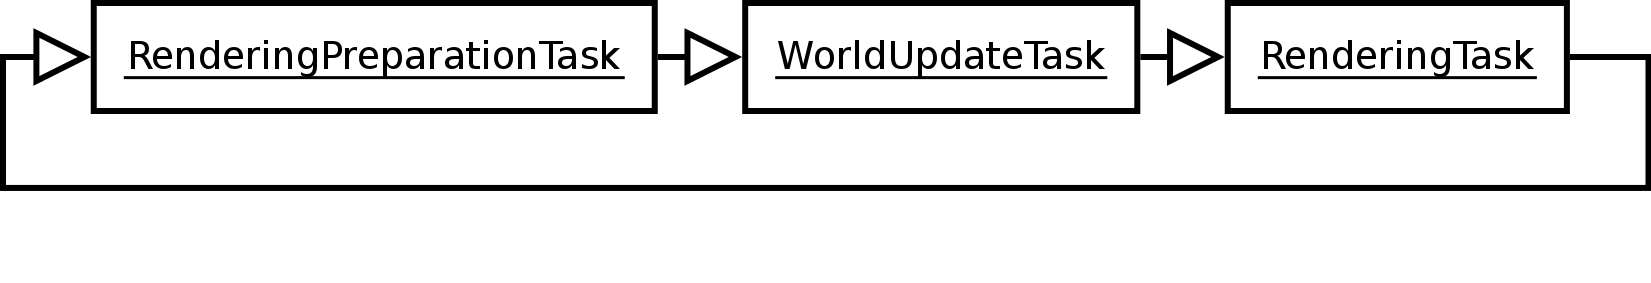
\includegraphics[width=12cm]{images/TaskQueue.png}
			\caption{A very simple rendering loop.}
			\label{fig:TaskQueue}
		\end{figure}

